\vspace*{-1cm}

\nombreCapituloCabecera{RH}{Fundamentos teóricos}

\section{Fundamentos teóricos}
\label{sec:fundamentos_teoricos}

El desarrollo de un laboratorio orientado a ejercicios de Red Team requiere comprender los principales conceptos, vulnerabilidades y técnicas empleados tanto por atacantes como por profesionales de la seguridad ofensiva. Este capítulo presenta los fundamentos teóricos necesarios para entender los escenarios implementados posteriormente en el laboratorio y las distintas fases de explotación desarrolladas durante las pruebas de validación.

Se describen las principales categorías de vulnerabilidades utilizadas en la aplicación web, los conceptos asociados a infraestructuras Active Directory, así como las técnicas de pivoting, movimiento lateral y escalada de privilegios empleadas durante los ejercicios prácticos.

% ---------------------------------------------------

\subsection{OWASP Top 10}

OWASP Top 10 es uno de los estándares de referencia más utilizados para clasificar los riesgos de seguridad más relevantes presentes en aplicaciones web. Publicado periódicamente por la organización Open Worldwide Application Security Project (OWASP), recopila las categorías de vulnerabilidades que generan un mayor impacto sobre la seguridad de aplicaciones reales\footweb{owasp_top10_2025}.

La edición de 2025 mantiene \textit{Broken Access Control} como la categoría de riesgo más crítica e introduce cambios significativos respecto a versiones anteriores, como la incorporación de \textit{Software Supply Chain Failures} o la nueva categoría \textit{Mishandling of Exceptional Conditions}. Asimismo, categorías clásicas como \textit{Injection}, \textit{Security Misconfiguration} o \textit{Authentication Failures} continúan ocupando posiciones destacadas dentro de la clasificación.

En este proyecto, OWASP Top 10 se utiliza como marco de referencia para seleccionar las vulnerabilidades implementadas en el portal vulnerable. El objetivo no consiste en reproducir todas las categorías presentes en el estándar, sino aquellas que permiten construir una cadena de ataque realista dentro de un entorno corporativo tipo PYME.

\vspace{0.5cm}
\renewcommand{\arraystretch}{1.5}
\newcolumntype{C}[1]{>{\centering\arraybackslash}m{#1}}


\begin{table}[H]
    \centering
    \captionazul{Relación entre OWASP Top 10 2025 y vulnerabilidades implementadas en el laboratorio}

    \setlength{\arrayrulewidth}{0.3pt}

    \begin{tabular}{|C{1.4cm}|C{3cm}|C{5.8cm}|C{3cm}|}
        \hline
        \rowcolor{blue!10}
        \textbf{ID} & \textbf{Categoría OWASP 2025} & \textbf{Ejemplo en entorno PYME} & \textbf{Uso en el laboratorio} \\
        \hline
        \rowcolor{green!12}
        A01 & Broken Access Control & Acceso no autorizado a datos o funciones de otros usuarios & Implementada \\
        \hline
        \rowcolor{green!12}
        A02 & Security Misconfiguration & Servicios mal configurados, errores visibles o archivos sensibles expuestos & Implementada \\
        \hline
        A03 & Software Supply Chain Failures & Dependencias vulnerables o componentes externos comprometidos & No prioritaria \\
        \hline
        \rowcolor{green!12}
        A04 & Cryptographic Failures & Contraseñas débiles, hashes inseguros o datos sensibles mal protegidos & Implementada \\
        \hline
        \rowcolor{green!12}
        A05 & Injection & SQL Injection, XSS o inyección de comandos & Implementada \\
        \hline
        \rowcolor{green!12}
        A06 & Insecure Design & Flujos inseguros por falta de diseño seguro o threat modeling & Parcial \\
        \hline
        \rowcolor{green!12}
        A07 & Authentication Failures & Sesiones inseguras, credenciales débiles o reutilización de contraseñas & Implementada \\
        \hline
        A08 & Software or Data Integrity Failures & Falta de verificación de integridad en datos, código o actualizaciones & No prioritaria \\
        \hline
        \rowcolor{green!12}
        A09 & Security Logging \& Alerting Failures & Ausencia de registros o alertas ante acciones sospechosas & Parcial \\
        \hline
        \rowcolor{green!12}
        A10 & Mishandling of Exceptional Conditions & Errores que revelan rutas, consultas, stack traces o información interna & Implementada \\
        \hline
    \end{tabular}

    \renewcommand{\arraystretch}{1}
    \label{tab:owasp_top10_laboratorio}
\end{table}
\vspace{0.5cm}


Las categorías marcadas en verde corresponden a vulnerabilidades que han sido implementadas total o parcialmente durante el diseño del laboratorio. Su selección responde a criterios de realismo, relevancia práctica y capacidad para encadenar diferentes fases de explotación dentro de un escenario ofensivo completo.

En primer lugar, las vulnerabilidades de control de acceso, autenticación e inyección permiten reproducir el acceso inicial al entorno. En segundo lugar, las configuraciones inseguras, fallos criptográficos y exposición de credenciales facilitan la transición hacia fases de post-explotación. Finalmente, la gestión deficiente de errores y la falta de registro o alerta permiten simular situaciones en las que el atacante puede avanzar sin ser detectado con facilidad.

Por tanto, OWASP Top 10 no se utiliza únicamente como una lista de vulnerabilidades aisladas, sino como una guía para seleccionar debilidades que puedan encadenarse dentro de un escenario ofensivo completo.
% ---------------------------------------------------

\subsection{MITRE ATT\&CK}

MITRE ATT\&CK (\textit{Adversarial Tactics, Techniques and Common Knowledge}) es una base de conocimiento desarrollada por MITRE Corporation que documenta tácticas y técnicas empleadas por atacantes reales durante operaciones ofensivas sobre sistemas informáticos\footweb{mitre_attack}.

A diferencia de OWASP Top 10, cuyo enfoque se centra principalmente en vulnerabilidades presentes en aplicaciones web, MITRE ATT\&CK permite modelar el comportamiento del atacante una vez que se ha iniciado el proceso de compromiso. Para ello organiza las técnicas ofensivas en distintas tácticas que representan objetivos concretos dentro de una intrusión.

En este trabajo, MITRE ATT\&CK se utiliza como referencia para relacionar las diferentes fases del laboratorio con técnicas ampliamente reconocidas por la comunidad de ciberseguridad. De este modo, actividades como la explotación web, la obtención de una reverse shell, la escalada de privilegios o el movimiento lateral pueden asociarse con tácticas descritas dentro del marco ATT\&CK.

\begin{figure}[H]
    \centering

    \begin{tikzpicture}[
        node distance=0.5cm,
        tactical/.style={
            rectangle,
            rounded corners,
            draw=blueColor,
            fill=blue!10,
            minimum width=2cm,
            minimum height=1.2cm,
            align=center,
            font=\footnotesize
        },
        flecha/.style={
            -{Latex[length=2mm]},
            thick
        }
    ]

    \node[tactical] (initial) {Initial\\Access};
    \node[tactical, right=of initial] (execution) {Execution};
    \node[tactical, right=of execution] (priv) {Privilege\\Escalation};
    \node[tactical, right=of priv] (cred) {Credential\\Access};
    \node[tactical, right=of cred] (disc) {Discovery};
    \node[tactical, right=of disc] (lateral) {Lateral\\Movement};

    \draw[flecha] (initial) -- (execution);
    \draw[flecha] (execution) -- (priv);
    \draw[flecha] (priv) -- (cred);
    \draw[flecha] (cred) -- (disc);
    \draw[flecha] (disc) -- (lateral);

    \end{tikzpicture}

    \vspace{0.3cm}
    \captionazul{Tácticas MITRE ATT\&CK relacionadas con la cadena de ataque del laboratorio.}
    \label{fig:mitre_attack_resumido}
\end{figure}

La Figura~\ref{fig:mitre_attack_resumido} resume las tácticas ATT\&CK más relevantes para los escenarios desarrollados en el laboratorio. Estas fases permiten relacionar la explotación práctica realizada durante el TFM con una taxonomía ampliamente utilizada en ejercicios de Red Team, análisis de amenazas y respuesta ante incidentes.

% ---------------------------------------------------

\subsection{SQL Injection}

La inyección SQL (\textit{SQL Injection} o SQLi) es una vulnerabilidad de inyección que aparece cuando una aplicación construye consultas SQL utilizando datos proporcionados por el usuario sin aplicar controles adecuados de validación, parametrización o separación entre datos e instrucciones. OWASP la identifica como una de las vulnerabilidades clásicas dentro de la categoría de inyección\footweb{owasp_sqli_prevention}.

Un atacante puede aprovechar este fallo para modificar la lógica de una consulta legítima y acceder a información no autorizada, alterar datos almacenados o, en determinados escenarios, realizar acciones administrativas sobre la base de datos. La guía de pruebas de OWASP incluye SQL Injection dentro de las técnicas de validación de entrada más relevantes para aplicaciones web\footweb{owasp_wstg_sqli}.

En el contexto de este laboratorio, SQL Injection se utiliza como uno de los posibles vectores de acceso inicial al sistema. Su inclusión permite simular un fallo frecuente en aplicaciones corporativas donde formularios de autenticación, búsqueda o consulta interactúan directamente con una base de datos.

% ---------------------------------------------------

\subsection{Cross-Site Scripting (XSS)}

Cross-Site Scripting (XSS) es una vulnerabilidad que permite introducir código JavaScript no confiable en una página web, de forma que este pueda ejecutarse en el navegador de otros usuarios. OWASP destaca que este tipo de vulnerabilidad puede permitir la ejecución de acciones en nombre de la víctima, el robo de información sensible o la modificación del contenido mostrado por la aplicación\footweb{owasp_xss_prevention}.

Estas vulnerabilidades aparecen cuando una aplicación muestra datos proporcionados por el usuario sin aplicar mecanismos adecuados de validación y codificación de salida. Dependiendo de su funcionamiento, OWASP distingue diferentes variantes, entre las que destacan el XSS reflejado, el XSS almacenado y el XSS basado en DOM\footweb{owasp_xss_types}.

Dentro del laboratorio, XSS se utiliza para representar un fallo habitual en portales web donde existen formularios, campos de entrada o funcionalidades de gestión de contenido. Su implementación permite analizar el impacto de no tratar correctamente los datos introducidos por los usuarios y estudiar cómo una vulnerabilidad de cliente puede afectar a la seguridad global de la aplicación.
% ---------------------------------------------------

\subsection{Vulnerabilidades de carga de archivos (File Upload)}

Las funcionalidades de carga de archivos (\textit{File Upload}) constituyen una superficie de ataque habitual en aplicaciones web modernas, especialmente en portales corporativos que permiten adjuntar documentos, imágenes o evidencias a formularios internos.

Cuando una aplicación no valida correctamente los archivos recibidos, un atacante puede subir contenido malicioso con el objetivo de ejecutar código en el servidor, almacenar ficheros peligrosos o comprometer a otros usuarios del sistema. OWASP destaca que este tipo de funcionalidad debe validar aspectos como la extensión, el tipo MIME, el tamaño, el nombre del archivo y la ubicación final de almacenamiento\footweb{owasp_file_upload}.

En el contexto del laboratorio, esta vulnerabilidad permite representar un escenario realista en el que una funcionalidad aparentemente legítima, como la subida de documentos o adjuntos, puede convertirse en un vector de acceso inicial o facilitar fases posteriores de post-explotación.

% ---------------------------------------------------

\subsection{Exposición de credenciales}

La exposición accidental de credenciales constituye una de las causas habituales de compromiso en entornos corporativos. Este problema puede manifestarse mediante archivos de configuración inseguros, copias de seguridad accesibles, credenciales embebidas en código fuente, variables de entorno expuestas o contraseñas almacenadas sin mecanismos de protección adecuados.

OWASP incluye la protección de datos sensibles y secretos dentro de sus recomendaciones de seguridad, especialmente cuando una aplicación maneja credenciales, claves, tokens o información de autenticación reutilizable\footweb{owasp_secrets_management}.

Una vez obtenidas, estas credenciales permiten a un atacante acceder a nuevos sistemas y ampliar progresivamente el alcance de una intrusión. En entornos reales, la reutilización de contraseñas entre servicios incrementa significativamente el impacto, ya que una credencial comprometida puede servir para acceder a sistemas internos, bases de datos, servicios administrativos o recursos compartidos.

Dentro del laboratorio, la exposición de credenciales se utiliza como mecanismo para conectar la explotación web inicial con fases posteriores de escalada, pivoting y movimiento lateral.

% ---------------------------------------------------

\subsection{Escalada de privilegios en Linux}

La escalada de privilegios engloba el conjunto de técnicas utilizadas para obtener permisos superiores a los inicialmente concedidos a un usuario comprometido. En sistemas Linux, estas técnicas suelen aprovechar configuraciones inseguras, permisos excesivos sobre ficheros, tareas programadas, binarios con privilegios elevados o scripts administrativos mal diseñados.

Desde el punto de vista de MITRE ATT\&CK, la escalada de privilegios constituye una táctica propia cuyo objetivo es obtener un nivel de acceso superior dentro del sistema comprometido\footweb{mitre_privilege_escalation}.

En el laboratorio, esta fase permite transformar un acceso inicial limitado sobre el servidor Ubuntu en un control completo del sistema. Esto resulta fundamental para continuar la cadena ofensiva, ya que permite acceder a información interna, modificar configuraciones, preparar mecanismos de pivoting y obtener credenciales útiles para comprometer otros sistemas de la infraestructura.

% ---------------------------------------------------

\subsubsection{PATH Hijacking}

\textit{PATH Hijacking} es una técnica de escalada de privilegios que aprovecha configuraciones inseguras relacionadas con la variable de entorno \texttt{PATH}. Esta variable define los directorios en los que el sistema busca ejecutables cuando se invoca un comando sin indicar su ruta absoluta.

El riesgo aparece cuando un script o programa ejecutado con privilegios elevados llama a comandos del sistema sin utilizar rutas absolutas. En ese caso, un atacante puede situar un ejecutable malicioso con el mismo nombre en un directorio controlado y modificar el orden de búsqueda de \texttt{PATH} para que dicho ejecutable sea invocado antes que el binario legítimo. La documentación de GNU Bash describe el uso de variables de entorno como \texttt{PATH} y su influencia en la ejecución de comandos dentro del intérprete\footweb{gnu_bash_manual}.

En el laboratorio, esta técnica se utiliza como ejemplo de escalada de privilegios local sobre el servidor Linux comprometido. Su inclusión permite mostrar cómo una mala práctica aparentemente sencilla en un script administrativo puede transformar un acceso limitado en un compromiso completo del sistema.

% ---------------------------------------------------

\subsubsection{Configuraciones inseguras}

Las configuraciones inseguras representan una categoría amplia de vulnerabilidades derivadas de errores administrativos, valores por defecto inseguros o decisiones de configuración incorrectas. Este tipo de debilidad no siempre se debe a un fallo del software, sino a la forma en la que los servicios, permisos o mecanismos de autenticación han sido desplegados.

Entre los ejemplos más habituales se encuentran permisos excesivos sobre archivos, servicios innecesarios habilitados, credenciales por defecto, exposición de directorios sensibles, errores de configuración en servidores web o ausencia de cabeceras de seguridad. OWASP considera \textit{Security Misconfiguration} una de las categorías principales dentro de los riesgos de seguridad en aplicaciones web y destaca que puede afectar tanto a la aplicación como a servidores, bases de datos, frameworks o servicios de infraestructura\footweb{owasp_top10_2025}.

Dentro del laboratorio, las configuraciones inseguras se introducen de forma controlada para aumentar la superficie de ataque y facilitar la construcción de cadenas de explotación realistas. Este tipo de debilidad permite conectar vulnerabilidades web con fases posteriores de post-explotación, escalada de privilegios o acceso a información sensible.

% ---------------------------------------------------

\subsection{Pivoting y segmentación de red}

El \textit{pivoting} es una técnica utilizada para acceder a sistemas o redes que inicialmente no son alcanzables directamente desde la posición del atacante. Para ello, se utiliza un sistema previamente comprometido como punto intermedio desde el que redirigir tráfico, crear túneles o alcanzar segmentos internos de la red.

Esta técnica resulta especialmente relevante en entornos corporativos segmentados, donde los sistemas internos no suelen estar expuestos directamente al exterior. MITRE ATT\&CK recoge distintas técnicas relacionadas con el uso de proxies, túneles y mecanismos de red para canalizar comunicaciones a través de sistemas intermedios comprometidos\footweb{mitre_proxy}.

En el contexto del laboratorio, el servidor Ubuntu vulnerable actúa como punto de apoyo tras el acceso inicial. Una vez comprometido, permite alcanzar la red interna donde se encuentran los sistemas Windows y la infraestructura Active Directory. De esta forma, el laboratorio permite reproducir una situación habitual en intrusiones reales: un servicio expuesto sirve como puerta de entrada hacia sistemas internos protegidos mediante segmentación de red.

\begin{figure}[H]
    \centering
    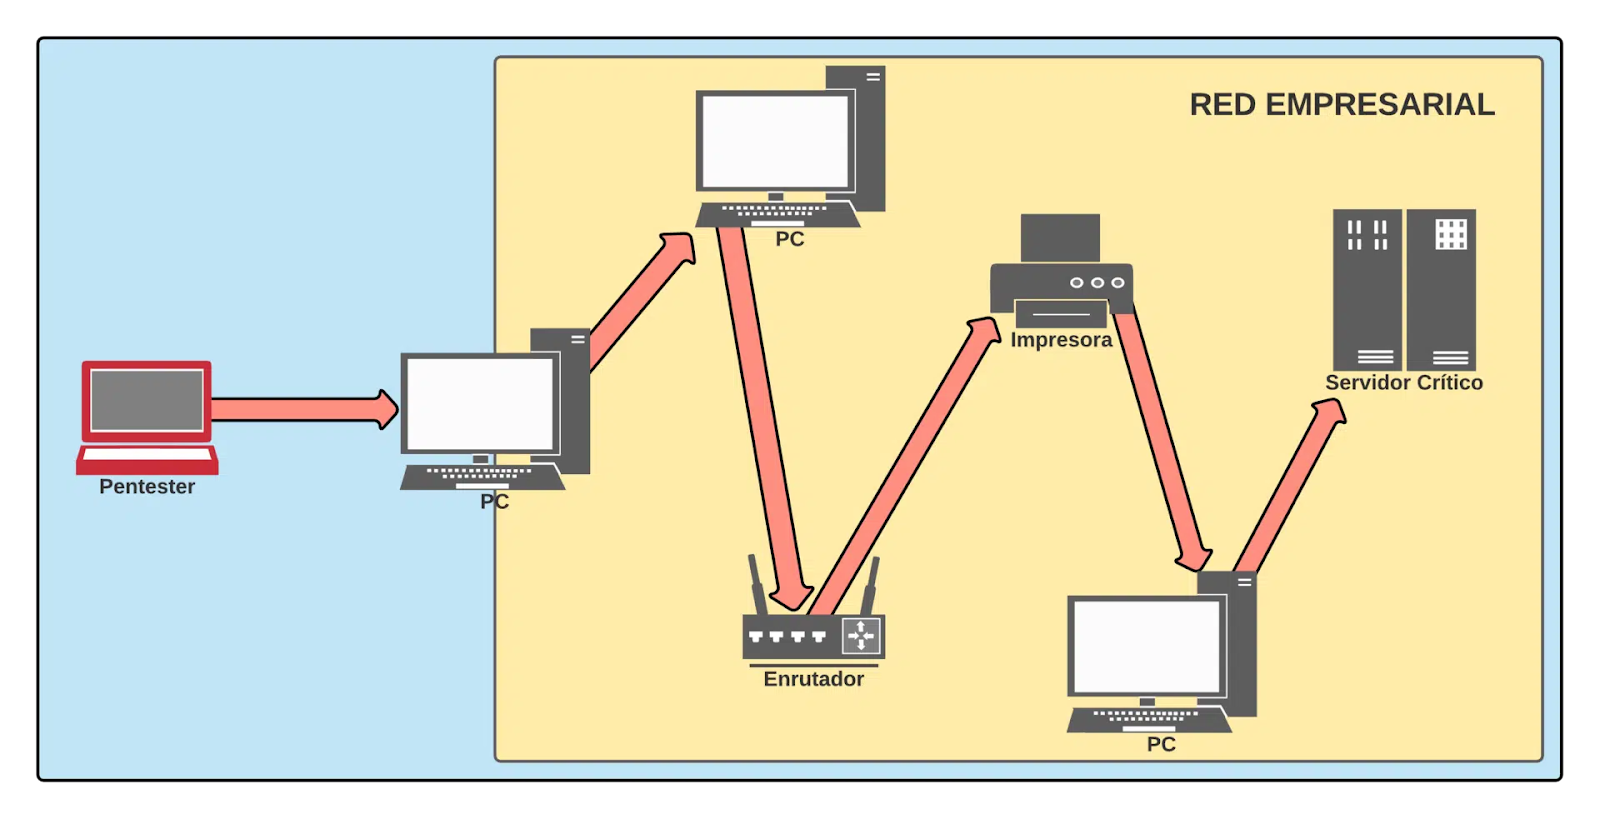
\includegraphics[width=0.9\textwidth]{Imagenes/FT-pivoting-segmentacion-redes.png}

    \vspace{0.2cm}
    \captionazul{Ejemplo conceptual de una operación de \textit{pivoting} sobre una red segmentada. Autor: \enlace{https://enfoqueseguro.com/enfoqueseguro/rafael-nunez-aponte-el-arte-del-pivoting-en-ciberseguridad/}{Rafael Núñez Aponte}.}

    \label{fig:fundamento_teorico_pivoting}
\end{figure}




% ---------------------------------------------------
% ---------------------------------------------------
% ---------------------------------------------------
% ---------------------------------------------------
\clearpage

\subsection{Active Directory}

\begin{figure}[H]
    \centering
    
\includegraphics[width=0.6\textwidth]{Imagenes/Active-Directory-logo.jpg}

    \vspace{0.2cm}
    \captionazul{Logotipo de Active Directory.}

    \label{fig:active_directory_logo}
\end{figure}

Active Directory Domain Services (AD DS) es el servicio de directorio de Microsoft utilizado para almacenar información sobre objetos de una red, como usuarios, equipos, grupos y otros recursos. Según la documentación oficial de Microsoft, AD DS proporciona una estructura jerárquica para organizar la información del directorio y hacerla accesible a usuarios y administradores autorizados\footweb{microsoft_ad_ds_overview}.

En entornos corporativos Windows, Active Directory permite centralizar la gestión de identidades, permisos y políticas, facilitando la administración de grandes cantidades de usuarios y equipos. Por este motivo, su compromiso puede tener un impacto elevado dentro de una organización, ya que un atacante con privilegios suficientes sobre el dominio puede acceder a recursos internos, modificar configuraciones o desplazarse hacia otros sistemas.

Dentro de este TFM, Active Directory se utiliza para simular una infraestructura corporativa realista, permitiendo desarrollar escenarios de enumeración, abuso de credenciales, movimiento lateral y compromiso de sistemas internos.

% ---------------------------------------------------

\subsubsection{Componentes principales}

Entre los componentes fundamentales de Active Directory destacan los dominios, bosques, unidades organizativas, controladores de dominio, cuentas de usuario, cuentas de equipo y grupos de seguridad. Microsoft describe la estructura lógica de Active Directory como un modelo jerárquico que permite organizar los recursos de acuerdo con necesidades administrativas, operativas y de delegación\footweb{microsoft_ad_logical_structure}.

Los controladores de dominio son los servidores encargados de almacenar la base de datos del directorio y proporcionar servicios de autenticación y autorización. Además, Active Directory se apoya en DNS para la localización de servicios y en Kerberos como mecanismo principal de autenticación dentro de dominios Windows. Microsoft documenta Kerberos como el protocolo utilizado para verificar la identidad de usuarios y hosts en entornos Windows Server\footweb{microsoft_kerberos_overview}.

En el laboratorio, estos componentes se simplifican mediante un único controlador de dominio, denominado \texttt{DC01}, y una estación de trabajo integrada en el dominio, denominada \texttt{DEV01}. Esta aproximación permite reproducir los elementos esenciales de un entorno corporativo sin incrementar excesivamente la complejidad del despliegue.

% ---------------------------------------------------

\subsubsection{Usuarios, grupos y permisos}

La gestión de permisos dentro de Active Directory se basa principalmente en cuentas de usuario, cuentas de equipo y grupos de seguridad. Los grupos permiten agrupar identidades y asignar permisos de forma centralizada sobre recursos compartidos, simplificando la administración frente a la asignación individual de permisos\footweb{microsoft_ad_security_groups}.

Este modelo facilita la gestión de entornos corporativos, pero también introduce riesgos cuando existen configuraciones incorrectas, privilegios excesivos o pertenencias indebidas a grupos administrativos. Microsoft identifica determinadas cuentas y grupos privilegiados de Active Directory como elementos especialmente sensibles, ya que disponen de permisos elevados para realizar acciones administrativas sobre el dominio y los sistemas unidos a él\footweb{microsoft_ad_privileged_accounts}.

En el contexto del laboratorio, la existencia de diferentes usuarios, grupos y niveles de privilegio permite simular escenarios en los que un atacante obtiene credenciales válidas y las reutiliza para acceder a otros sistemas, enumerar recursos o realizar movimiento lateral dentro de la infraestructura.

% ---------------------------------------------------
\subsection{Protocolos y servicios utilizados}

Diversos protocolos de red desempeñan un papel fundamental dentro de los entornos Windows modernos y suelen constituir objetivos habituales durante las fases de enumeración y post-explotación.

En este laboratorio destacan especialmente los servicios asociados a Active Directory, DNS, SMB y WinRM. Estos protocolos permiten reproducir operaciones habituales de una red corporativa, como la resolución de nombres, la autenticación centralizada, la compartición de recursos y la administración remota de sistemas. Al mismo tiempo, proporcionan una superficie de análisis relevante para estudiar técnicas de enumeración, abuso de credenciales y movimiento lateral.

Desde el punto de vista ofensivo, estos servicios resultan relevantes porque pueden proporcionar información sobre usuarios, equipos, recursos compartidos o mecanismos de acceso remoto. Por ello, su presencia en el laboratorio permite conectar la parte teórica de la infraestructura Windows con los escenarios prácticos de explotación desarrollados posteriormente.

% ---------------------------------------------------

\subsubsection{SMB}

Server Message Block (SMB) es un protocolo de compartición de archivos utilizado en entornos Windows para acceder a ficheros, impresoras y otros recursos a través de la red. Microsoft lo describe como un protocolo de uso compartido de archivos que permite a las aplicaciones leer, crear y actualizar archivos en servidores remotos\footweb{microsoft_smb_overview}.

Su amplia utilización en redes corporativas lo convierte en una fuente importante de información durante las fases de reconocimiento y enumeración. A través de SMB pueden identificarse recursos compartidos, permisos de acceso, nombres de equipos o información útil para fases posteriores del ataque.

En el contexto del laboratorio, SMB permite simular la compartición de recursos internos dentro de la infraestructura Windows y sirve como superficie de análisis durante las fases de enumeración y movimiento lateral.

% ---------------------------------------------------

\subsubsection{WinRM}

Windows Remote Management (WinRM) es la implementación de Microsoft del protocolo WS-Management, diseñado para permitir la administración remota de sistemas Windows mediante un protocolo interoperable y compatible con distintos entornos\footweb{microsoft_winrm_overview}.

En entornos corporativos, WinRM permite ejecutar tareas de administración remota y gestionar equipos Windows de forma centralizada. Desde una perspectiva ofensiva, cuando un atacante dispone de credenciales válidas, este servicio puede utilizarse para obtener acceso remoto interactivo a sistemas comprometidos y ejecutar comandos sobre ellos.

Dentro del laboratorio, WinRM se utiliza para representar un mecanismo de administración remota habitual en infraestructuras Windows. Su inclusión permite estudiar cómo las credenciales obtenidas durante fases anteriores pueden emplearse para acceder a equipos internos y avanzar en la cadena de ataque.

% ---------------------------------------------------

\subsection{Movimiento lateral en entornos Windows}

El movimiento lateral engloba el conjunto de técnicas utilizadas por un atacante para desplazarse entre diferentes sistemas dentro de una infraestructura comprometida. MITRE ATT\&CK define esta táctica como el conjunto de técnicas utilizadas para entrar y controlar sistemas remotos dentro de una red\footweb{mitre_lateral_movement}.

Estas técnicas suelen apoyarse en credenciales obtenidas previamente, relaciones de confianza existentes entre equipos, servicios de administración remota o configuraciones inseguras presentes en el dominio. En entornos Windows, protocolos como SMB y WinRM pueden desempeñar un papel relevante, ya que permiten acceder a recursos compartidos o ejecutar acciones de administración remota.

En entornos Active Directory, el movimiento lateral constituye una fase crítica de la intrusión. Permite al atacante progresar desde sistemas de bajo privilegio hacia recursos de mayor criticidad, como estaciones de trabajo internas, servidores corporativos o controladores de dominio. Por este motivo, el laboratorio incorpora una infraestructura Windows que permite reproducir este tipo de técnicas en un entorno controlado.
